\documentclass[a4paper]{article}

%use the english line for english reports
%usepackage[english]{babel}
\usepackage[portuguese]{babel}
\usepackage[utf8]{inputenc}
\usepackage{indentfirst}
\usepackage{graphicx}
\usepackage{verbatim}
\usepackage{listings}


\begin{document}

\setlength{\textwidth}{16cm}
\setlength{\textheight}{22cm}

\title{\Huge\textbf{Ni-ju}\linebreak\linebreak\linebreak
\Large\textbf{Relatório Intercalar}\linebreak\linebreak
\linebreak\linebreak

\includegraphics[scale=0.1]{../printscreens/feup-logo.png}\linebreak\linebreak
\linebreak\linebreak
\Large{Mestrado Integrado em Engenharia Informática e Computação} \linebreak\linebreak
\Large{Programação em Lógica}\linebreak
}

\author{\textbf{Grupo xx:}\\
Nome1 - Número1 \\
João Pedro Furriel de Moura Pinheiro - up201104913\\
Ventura de Sousa Pereira - up201404690\\
\linebreak\linebreak \\
 \\ Faculdade de Engenharia da Universidade do Porto \\ Rua Roberto Frias, s\/n, 4200-465 Porto, Portugal \linebreak\linebreak\linebreak
\linebreak\linebreak\vspace{1cm}}

\maketitle
\thispagestyle{empty}

%************************************************************************************************
%************************************************************************************************

\newpage

%Todas as figuras devem ser referidas no texto. %\ref{fig:codigoFigura}
%
%%Exemplo de código para inserção de figuras
%%\begin{figure}[h!]
%%\begin{center}
%%escolher entre uma das seguintes três linhas:
%%\includegraphics[height=20cm,width=15cm]{path relativo da imagem}
%%\includegraphics[scale=0.5]{path relativo da imagem}
%%\includegraphics{path relativo da imagem}
%%\caption{legenda da figura}
%%\label{fig:codigoFigura}
%%\end{center}
%%\end{figure}
%
%
%\textit{Para escrever em itálico}
%\textbf{Para escrever em negrito}
%Para escrever em letra normal
%``Para escrever texto entre aspas''
%
%Para fazer parágrafo, deixar uma linha em branco.
%
%Como fazer bullet points:
%\begin{itemize}
	%\item Item1
	%\item Item2
%\end{itemize}
%
%Como enumerar itens:
%\begin{enumerate}
	%\item Item 1
	%\item Item 2
%\end{enumerate}
%
%\begin{quote}``Isto é uma citação''\end{quote}


%%%%%%%%%%%%%%%%%%%%%%%%%%
\section{O Jogo Ni-ju}

Ni-ju (traduzido para 20, em japonês) é um jogo que desenvolvido pelo designer e artista Néstor Romeral Andrés e artista, em 2016, tendo sido publicado pela HenMar Games, nestorgames.
O jogo é constituido por 40 peças, sendo estas divididas por cor - branca e preta, entre os jogadores, ficando, cada um, com 20 peças de padrões diferentes (daí o nome do jogo). Será possivel ter 70 padrões diferentes, se incluirmos rotações.
Para comelar, cada jogador deverá colocar uma peça na zona de jogo, seguido pelo seu adversário, até as condições de vitória se reunirem.
O objetivo do jogo é recriar o padrão descrito na peça, à volta da mesma. No final ganha quem conseguir recriar mais padrões, quando se esgotarem as peças.
\linebreak\linebreak\\
\textbf{Regra}:
Regra do Posionamento: 
  Aquando a vez de um jogador, o mesmo apenas poderá colocar a sua peça adjacente a uma das já jogadas.
\linebreak\linebreak\\

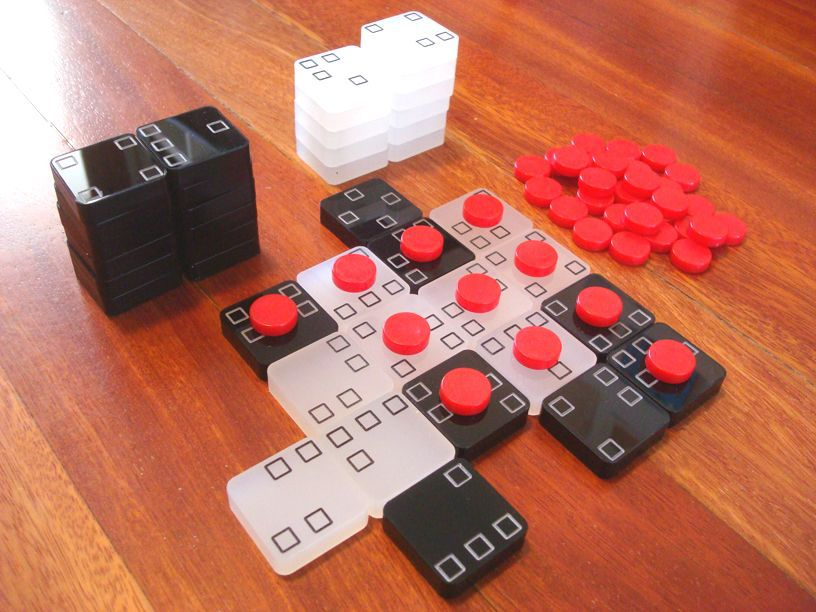
\includegraphics[scale=0.3]{../printscreens/niju.jpg} \linebreak
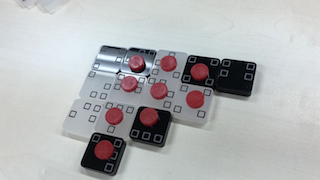
\includegraphics[scale=0.5]{../printscreens/niju2.png} \linebreak

Devem ser incluidas as fontes de informação (e.g. URLs em rodapé).


%%%%%%%%%%%%%%%%%%%%%%%%%%
\section{Representação do Estado do Jogo}

Inicialmente, o estado inicial do jogo será uma lista vazia [], visto que este é dinâmico. Modifica-se conforme a posição de cada peça jogada.

\textbf{Estado Inicial}:

[
  [
      [[-1, -1, -1],
		  [-1, -1, -1],
		  [-1, -1, -1]
		 ]
                      ]
	                 ]\linebreak\linebreak\\

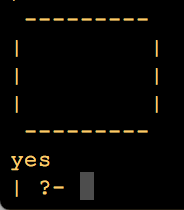
\includegraphics[scale=0.8]{../printscreens/initial_board.png} \linebreak


Num estado intermédio, o jogo terá algumas peças em jogo, constituindo a constituição doo mesmo.

\textbf{Possível representação}:

	[
		%row1
		[

		 [[0, 1, 1],
		  [0, 0, 1],
		  [0, 0, 1]
		 ],

		 [[0, 2, 2],
		  [0, 0, 0],
		  [2, 0, 2]
		 ]

		],

		%row2

		[

		 [[-1, -1, -1],
		  [-1, -1, -1],
		  [-1, -1, -1]
		 ],

		 [[1, 0, 1],
		  [0, 0, 0],
		  [1, 0, 1]
		 ]

		]
		
	]\linebreak\linebreak\\

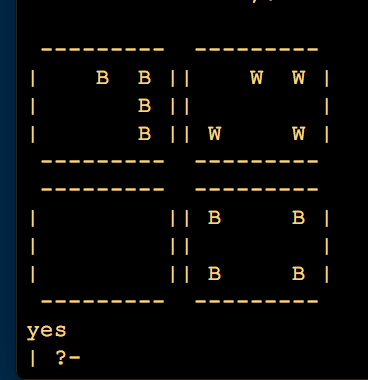
\includegraphics[scale=0.8]{../printscreens/intermediate_board.png} \linebreak

Objetos P1 serão as peças, que, por sua vez, são uma matriz (lista de listas), cuja representação poderá ser:

[[1,1,1],
[0,0,1],
[0,0,0]]

\textbf{Representação final}:

[

		%row1

		[

		 [[2, 0, 0],
		  [2, 0, 0],
		  [2, 0, 2]
		 ],

		 [[2, 0, 0],
		  [0, 0, 2],
		  [0, 2, 2]
		 ],

		 [[0, 2, 0],
		  [0, 0, 0],
		  [2, 2, 2]
		 ],

		 [[1, 0, 0],
		  [1, 0, 0],
		  [1, 0, 1]
		 ]

		],


		%row2

		[

		 [[-1, -1, -1],
		  [-1, -1, -1],
		  [-1, -1, -1]
		 ],

		 [[2, 2, 2],
		  [0, 0, 2],
		  [0, 0, 0]
		 ],

		 [[0, 0, 2],
		  [2, 0, 2],
		  [2, 0, 0]
		 ],

		 [[0, 0, 1],
		  [1, 0, 1],
		  [1, 0, 0]
		 ]

		],

		%row3

		[

		 [[1, 0, 0],
		  [0, 0, 1],
		  [1, 1, 0]
		 ],

		 [[1, 1, 1],
		  [0, 0, 1],
		  [0, 0, 0]
		 ],

		 [[0, 0, 2],
		  [2, 0, 2],
		  [2, 0, 0]
		 ],

		 [[0, 0, 1],
		  [1, 0, 1],
		  [1, 0, 0]
		 ]

		]
		
	]\linebreak\linebreak\\

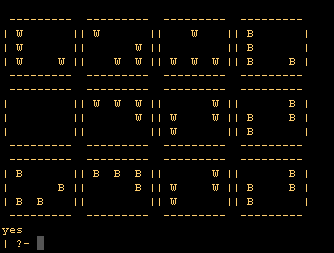
\includegraphics[scale=0.6]{../printscreens/winning_board.png} \linebreak




%%%%%%%%%%%%%%%%%%%%%%%%%%
\section{Visualização do Tabuleiro}

O padrão de cada peça é representado por B's ou W's, dependendo se a peça é preta ou branca, respetivamente. Os espaços vazios no tabuleiro são representados por uma matriz, de 3x3, de espaços. Além disso, os espaços vazios da peça são, também, representados por espaços.

\textbf{Predicados usados para a impressão do tabuleiro}:

printElement(X) :- X =:= 1, write(' B ').

printElement(X) :- X =:= 2, write(' W ').

printElement(X) :- X =:= -1, write('   ').

printElement(X) :- X =:= 0, write('   ').

printPieceRowSeparation(BoardRow) :-



	BoardRow = [].


\begin{lstlisting}
printPieceRowSeparation(BoardRow) :-
	
BoardRow \= [],

		 [\_ | Rest] = BoardRow,
	write(' --------- '),
	printPieceRowSeparation(Rest).

printPieceRow([X1,X2,X3]) :- 

write('|'),

    printElement(X1),
    printElement(X2),
    printElement(X3),
	write('|').


printBoard(Board) :-

	Board = [].

printBoard(Board) :- 

	[Row | Rest] = Board,

	printPieceRowSeparation(Row),
	nl,
	printPiecesRow1(Row),
	nl,
	printPiecesRow2(Row),
	nl,
	printPiecesRow3(Row),
	nl,
	printPieceRowSeparation(Row),
	nl,
	printBoard(Rest).

printPiecesRow1(BoardRow) :-

	BoardRow = [].

printPiecesRow1(BoardRow) :-

	[Piece | Rest] = BoardRow,
	[PieceRow1 | \_] = Piece,
	printPieceRow(PieceRow1),
	printPiecesRow1(Rest).


printPiecesRow2(BoardRow) :-
	BoardRow = [].

printPiecesRow2(BoardRow) :-
	[Piece | Rest] = BoardRow,
	[\_,PieceRow2,\_] = Piece,
	printPieceRow(PieceRow2),
	printPiecesRow2(Rest).


printPiecesRow3(BoardRow) :-

	BoardRow = [].

printPiecesRow3(BoardRow) :-

	[Piece | Rest] = BoardRow,
	[\_,\_,PieceRow3] = Piece,
	printPieceRow(PieceRow3),
	printPiecesRow3(Rest).
\end{lstlisting}


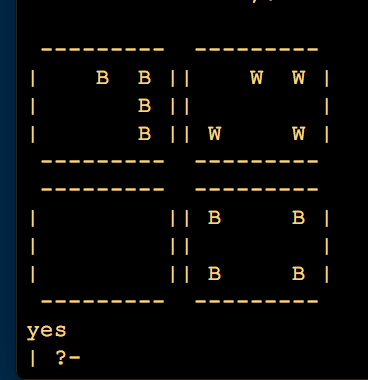
\includegraphics[scale=0.5]{../printscreens/intermediate_board.png} \linebreak

%%%%%%%%%%%%%%%%%%%%%%%%%%
\section{Movimentos}

Antes de cada jogada, os jogadores podem rodar as suas peças, para esse efeito os predicados a usar serão:

RotatePieceLeft(OldPiece, NewPiece)
RotatePieceright(OldPiece, NewPiece)

Depois da rotação os jogadores deverão posicionar as peças no tabuleiro numa posição adjacente a uma das peças já existentes no tabuleiro. Para tal, os predicados serão:

playPieceRight(CurrentBoard, Piece, Row, Column, ResultingBoard).
playPieceDown(CurrentBoard, Piece, Row, Column, ResultingBoard).
playPieceLeft(CurrentBoard, Piece, Row, Column, ResultingBoard).
playPieceUp(CurrentBoard, Piece, Row, Column, ResultingBoard).




\end{document}
